%%%%%%%%%%%%%%%%%%%%%%%%%%%%%%%%%%%%%%%%%%%%%%%%%%%%%%%%%%% Author - Varad Meru
%% tex source file for Homework 1.
%%%%%%%%%%%%%%%%%%%%%%%%%%%%%%%%%%%%%%%%%%%%%%%%%%%%%%%%%
\documentclass[a4paper, 11pt]{article}

\usepackage[margin=1in]{geometry} % changes the margin
\usepackage{lipsum} % adds random text to check the formatting
\usepackage{hyperref} % adds hyperlink
\usepackage[framed,numbered,autolinebreaks,useliterate]{mcode}
\usepackage{subfigure}
\usepackage{graphicx}
\usepackage{enumerate}

\renewcommand{\thefootnote}{\fnsymbol{footnote}} % Changes the format of the footnotes superscripts

%%%%%%%%%%%%%%%%%%%%%%%%%%%%%%%%%%%%%%%%%%%%%%%%%%%%%%%%%
\begin{document}
\begin{noindent}
\large\textbf{Week 2} \hfill \textbf{Varad Meru} \\
\normalsize CS 273a - Introduction to Machine Learning (Winter '15)\footnote{\href{http://sli.ics.uci.edu/Classes/2015W-273a}{Website: http://sli.ics.uci.edu/Classes/2015W-273a}} \hfill Student \# 26648958 \\
Prof. Alex Ihler \hfill Due Date: 01/20/2015
\end{noindent}
\noindent\makebox[\linewidth]{\rule{\textwidth}{0.4pt}}

%%%%%%%%%%%%%%%%%%%%%%%%%%%%%%%%%%%%%%%%%%%%%%%%%%%%%%%%%
%%%%%%%%%%%%%%%%%%%%%%%%%%%%%%%%%%%%%%%%%%%%%%%%%%%%%%%%%
\begin{center}
\textbf{\Large{Homework 2}\footnote{Questions available at \href{http://sli.ics.uci.edu/Classes/2015W-273a?action=download\&upname=HW2.pdf}{http://sli.ics.uci.edu/Classes/2015W-273a?action=download\&upname=HW2.pdf}}\footnote{All the figures and listing numbers are auto-refered.}}\\
\end{center}
\vspace{-25pt}

%%%%%%%%%%%%%%%%%%%%%%%%%%%%%%%%%%%%%%%%%%%%%%%%%%%%%%%%%
%%%%%%%%%%%%%%%%%%%%%%%%%%%%%%%%%%%%%%%%%%%%%%%%%%%%%%%%%
\section*{Problem 1: Linear Regression}
\begin{enumerate}[(a)]
\item I loaded the data from \texttt{data/curve80.data} into the \texttt{curve} variable. Then the variable \texttt{X} stores the data and \texttt{Y} stores the regressed values. I then split the data into a 75-25 partition and store it in the individual variables. Shown in \autoref{lst:curveLoad}.
\vspace{-15pt}
\begin{lstlisting}[caption={Fetching the \texttt{data/curve80.data} and splitting it with a 75-25 partition.},label={lst:curveLoad},numbers=left,escapeinside={@}{@}]
% Fetching the dataset and separating it into X and Y.
curve=load('data/curve80.txt');     % load the text file
y = curve(:,end);           % target value is last column
X = curve(:,1);       % features are other columns
whos

% Part (a)
% Splitting the data into 75-25 split.
[Xtr, Xte, Ytr, Yte] = splitData(X,y, .75);

>> whos
  Name        Size            Bytes  Class     Attributes

  X          80x1               640  double              
  Xte        20x1               160  double              
  Xtr        60x1               480  double              
  Yte        20x1               160  double              
  Ytr        60x1               480  double              
  curve      80x2              1280  double              
  y          80x1               640  double 
\end{lstlisting}

\item After loading the data, we use the \mcode{linearRegress} class's \mcode{predict()} to get the prediction of the model. The code is given in \autoref{lst:lr1}. The plot can be seen at \autoref{fig:lr1}.
\vspace{-15pt}
\begin{lstlisting}[caption={Getting a prediction for the model built on the Training data.},label={lst:lr1},numbers=left,escapeinside={@}{@}]
%% Part (b)
% Training the linear regression with Xtr as an input
lr = linearRegress( Xtr, Ytr );
xs = [0:.05:10]';
ys = predict(lr, xs);
ys1 = predict(lr, Xte);

% Plotting the training data and the predicted function in the same plot.
f=figure;
scatter(Xtr, Ytr, 'filled');
hold on;
plot(xs, ys);
hold off;
saveas(f,'lr.jpg','jpg');

% MSE for both Training and Test data
mse(lr, Xtr, Ytr)
% ans = 1.1277
mse(lr, Xte, Yte)
% ans = 2.2423
\end{lstlisting}

\begin{figure}
\centering
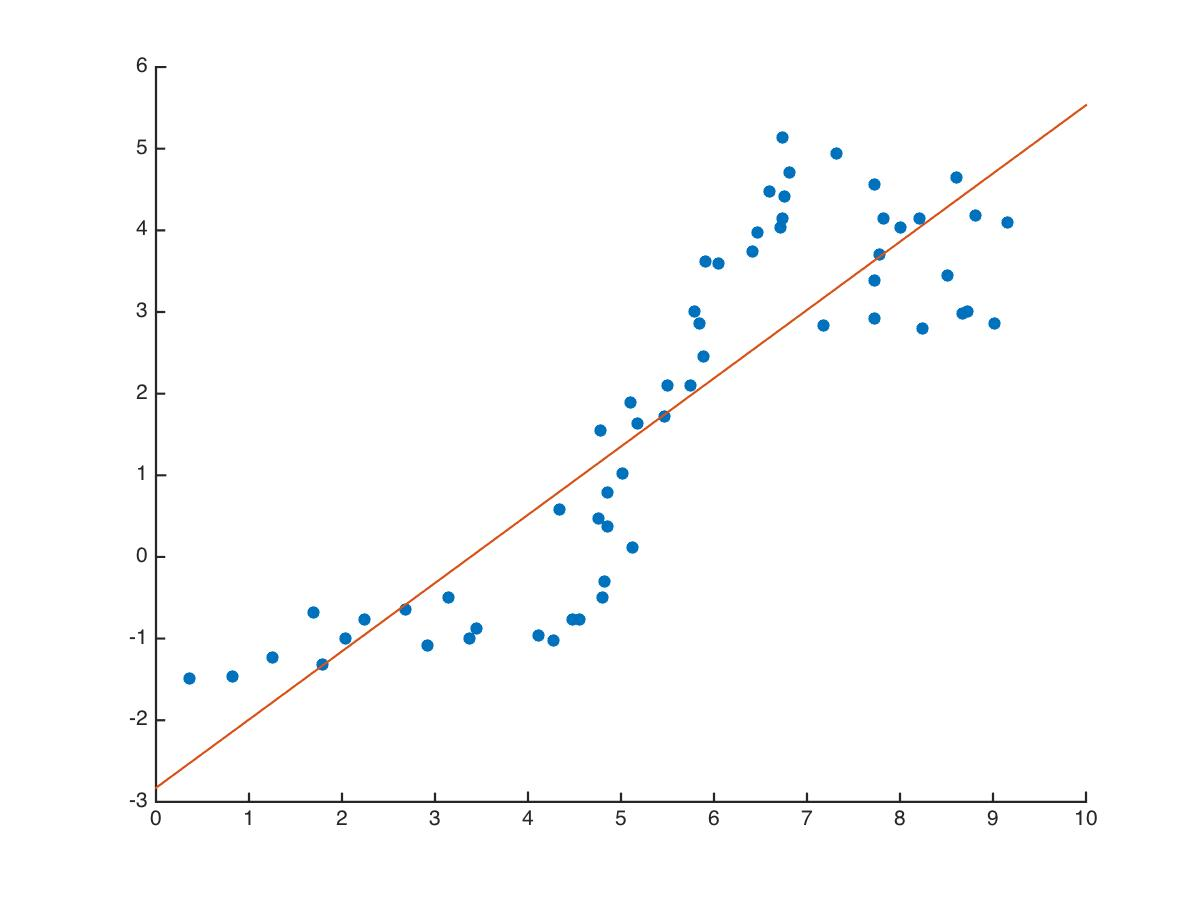
\includegraphics[scale=0.25]{lr.jpg}
\caption[lr1]{Training data and the learned function in \autoref{lst:lr1}}
\label{fig:lr1}
\end{figure}

\item The higher degree polynomials are created as per the \autoref{lst:lr2}. The higher-degree polynomials are created by the \mcode{fploy()} function provided. Using the new dataset, we rescale it and train the linear regression model using \mcode{linearRegress} class.
\vspace{-15pt}
\begin{lstlisting}[caption={Getting a prediction for the model built on the Training data.},label={lst:lr2},numbers=left,escapeinside={@}{@}]
f = figure;
i = 1;
errorsTr = zeros(1, 6);
errorsTe = zeros(1, 6);
d=[1,3,5,7,10,18];
for degree=[1,3,5,7,10,18];
    
    XtrP = fpoly(Xtr, degree, false); % create poly features up to given degree; no "1" feature.
    [XtrP, M,S] = rescale(XtrP); % it's often a good idea to scale the features 
    lr = linearRegress( XtrP, Ytr ); % create and train model
    
    % XS vs YS plot. 
    xs = [0:.05:10]';
    xsP = rescale( fpoly(xs,degree,false), M,S);
    ysP = predict( lr, xsP );
    
    % Scatter plot and the learned function on the data.
    subplot(2,3,i);
    title(strcat({'degree= '},num2str(degree)))
    hold on;
    scatter(Xtr, Ytr, 'filled');
    ax = axis;
    hold on;
    plot(xs, ysP);
    axis(ax);
    
    % For getting the right degree to get the best learning function.
    XteP = rescale(fpoly(Xte,degree,false), M,S);
    YteP = predict(lr,XteP);
    
    % MSE for both Training and Test data
    errorsTr(1, i) = mse(lr, XtrP, Ytr)
    errorsTe(1, i) = mse(lr, XteP, Yte)
    i= i+1;
    % now, apply the same polynomial expansion & scaling transformation to Xtest:
    % 
end;
hold off;
\end{lstlisting}

The trained functions and the scatter for various degree values can be seen in the visual representation seen in \autoref{fig:lr2}. To get to a better approximation of the right degree, we learned the performance of the learner with the test data and plotted it, as can be seen in \autoref{fig:lr3}. From this observation, I can see that for \textbf{degree = 10}, the test error was the least.
\begin{figure}
\centering
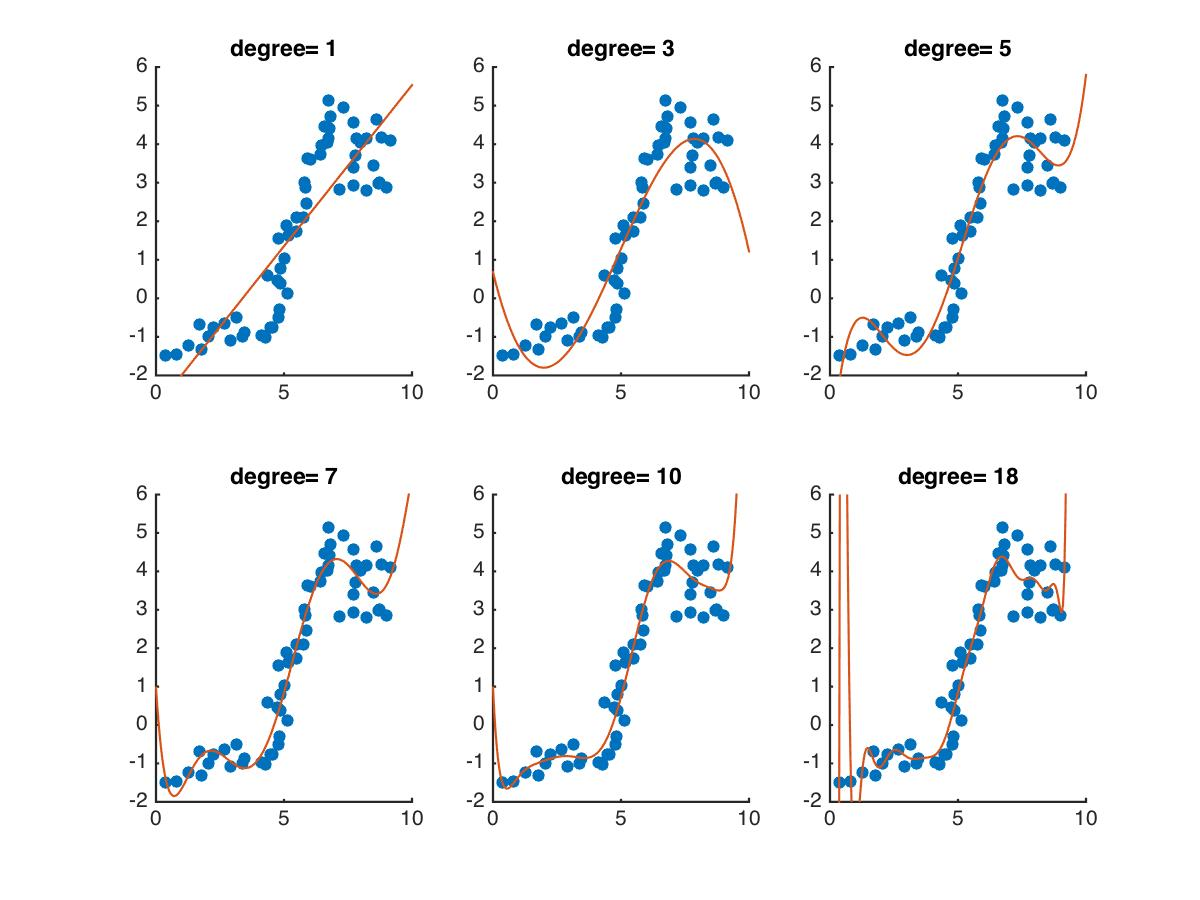
\includegraphics[scale=0.25]{lr1.jpg}
\caption[lr2]{Plots for different degree polynomials and the learned functions}
\label{fig:lr2}
\end{figure}

\begin{figure}
\centering
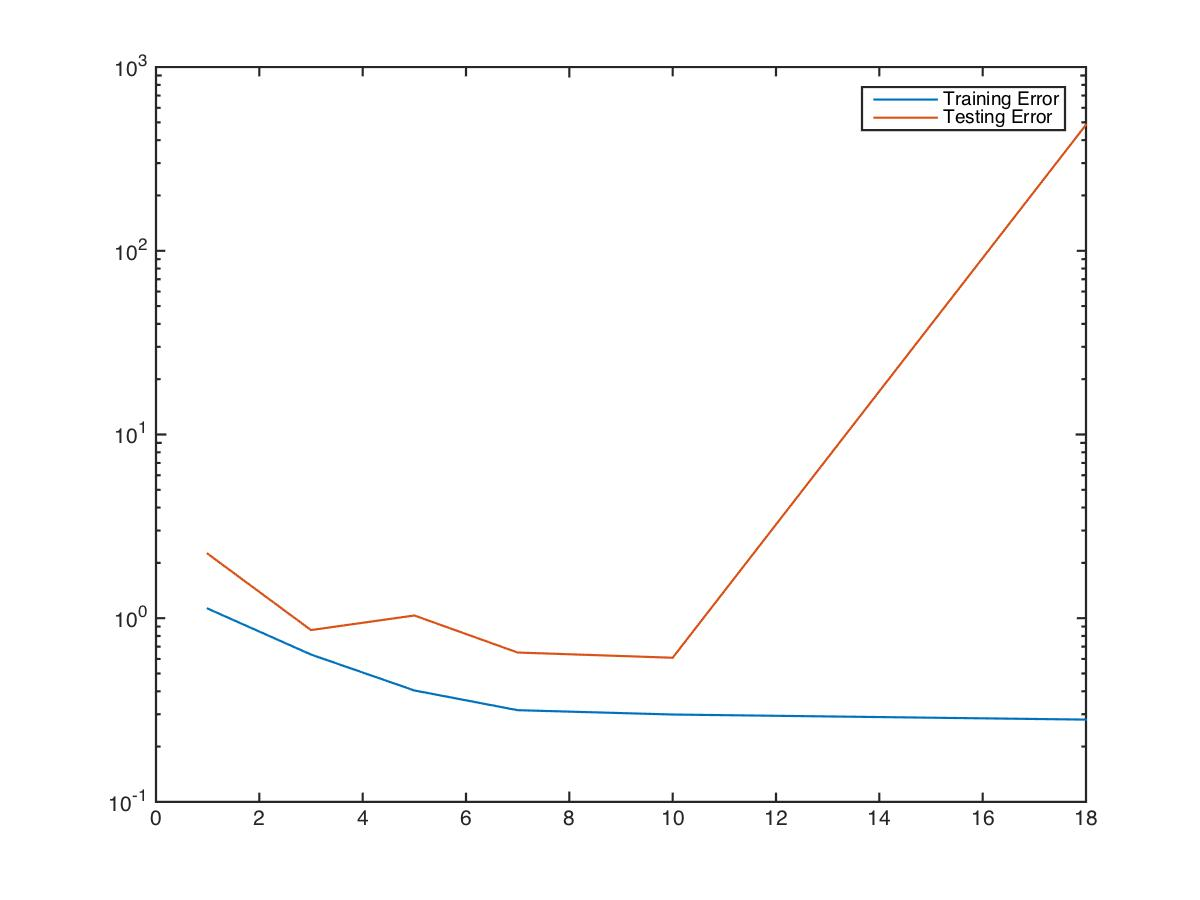
\includegraphics[scale=0.25]{lr2.jpg}
\caption[lr3]{Train and Test Errors.}
\label{fig:lr3}
\end{figure}

\end{enumerate}

%%%%%%%%%%%%%%%%%%%%%%%%%%%%%%%%%%%%%%%%%%%%%%%%%%%%%%%%%
%%%%%%%%%%%%%%%%%%%%%%%%%%%%%%%%%%%%%%%%%%%%%%%%%%%%%%%%%
\section*{Problem 2: Cross Validation}
\vspace{-10pt}
For each degree, I use cross validation within the loop iterating on all the degrees. Before I apply the cross-validation on this data and change its degree as well as rescale it, as seen in \autoref{lst:cv1}. After that, I  save the errors into an array and use that to plot, which can be seen in \autoref{fig:crossvala}. From this plot, it can be seen that for \textbf{degree = 5}, the error is minimum. When we compare it with the error on the actual test data, the difference shows up. The actual test data fits better for degree = 10, whereas cross validated data fits better with degree = 5. This plot shows that error for cross-validated model follows similar pattern to a test data, thus we can build models on data which would generalize better, without the knowledge of the actual test data.
\vspace{-15pt}
\begin{lstlisting}[caption={Training linear regression with cross-validation.},label={lst:cv1},numbers=left,escapeinside={@}{@}]
i = 1;
nFolds = 5;
d=[1,3,5,7,10,18];
for degree=[1,3,5,7,10,18];
    % Degrees and scaling of the data
    XtrP = fpoly(Xtr, degree, false); % create poly features up to given degree; no "1" feature.
    [XtrP, M,S] = rescale(XtrP); % it's often a good idea to scale the features 
    for iFold = 1:nFolds;
        [Xti,Xvi,Yti,Yvi] = crossValidate(XtrP,Ytr,nFolds,iFold);
        % take ith data block as v learner = linearRegress(... 
        lr = linearRegress( Xti, Yti ); % create and train model
        % TODO: train on Xti, Yti , the data for this fold J(iFold) = ... 
        
        % TODO: now compute the MSE on Xvi, Yvi and save it 
        J(iFold) = mse(lr, Xvi, Yvi);
    end;
    % the overall estimated validation performance is the average of the performance on ea
    errors(i) = mean(J);
    i = i + 1;
end;
\end{lstlisting}

\begin{figure}
\centering
\subfigure[Training Errors for various degrees when the data is cross-validated]{
    \label{fig:crossvala}
	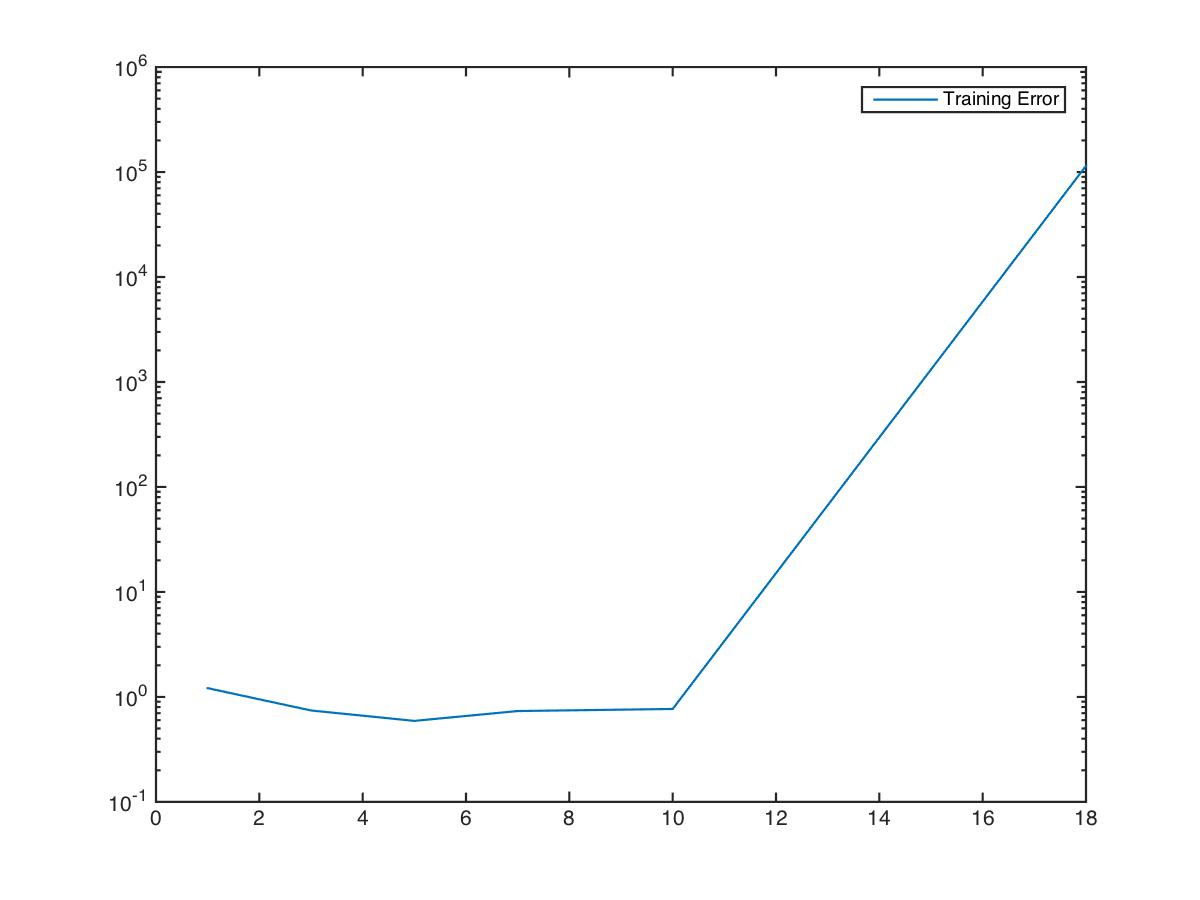
\includegraphics[scale=0.25]{cv.jpg}
}
\subfigure[Train Errors on Cross-validated error as well as the Error on the Actual Test data]{
    \label{fig:crossvalb}
	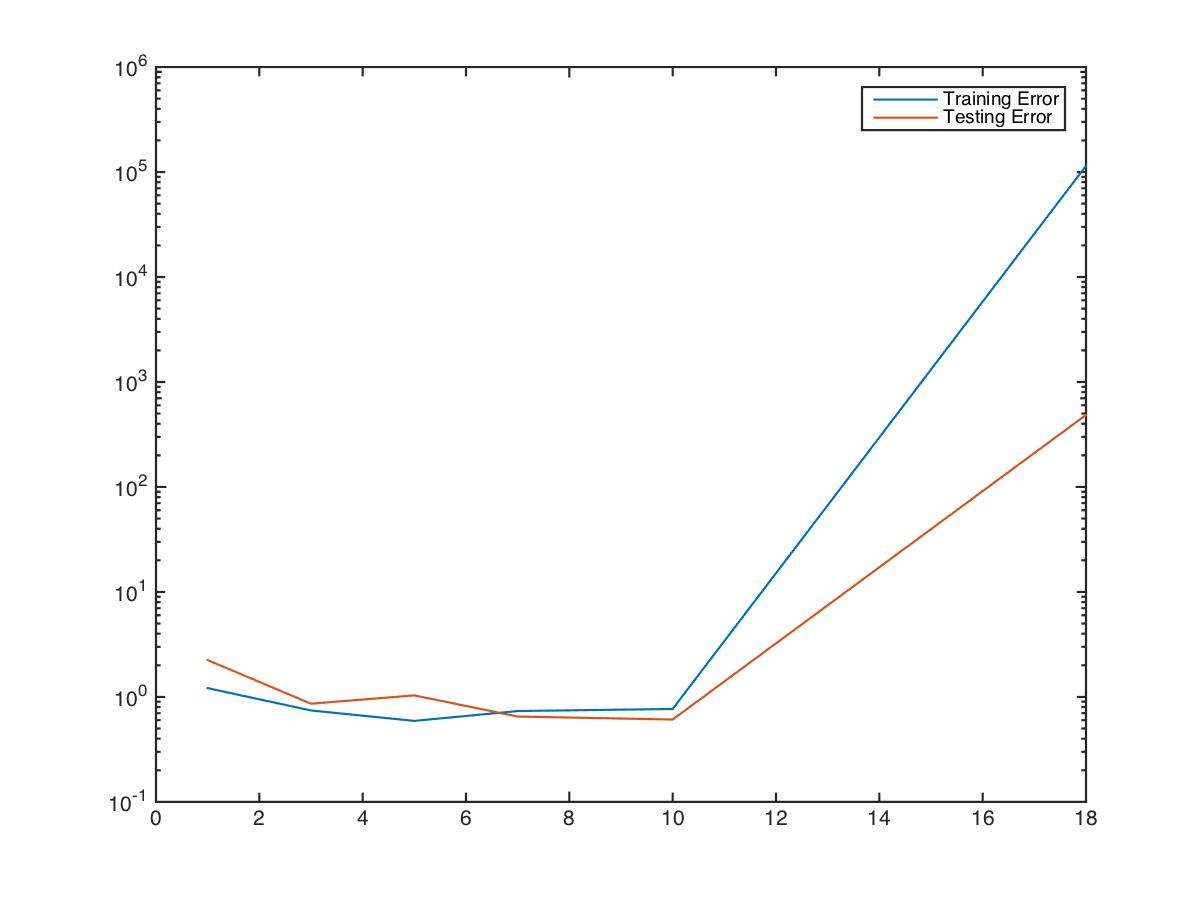
\includegraphics[scale=0.25]{cv1.jpg}
}
\caption[Running Various Experiments]{Running Various Experiments. The three bars are for Brute Force, I-Consistency and I-Consistency with MRV search. All the times given are in Seconds}
\label{fig:crossval}
\end{figure}
\end{document}

%%%%%%%%%%%%%%%%%%%%%%%%%%%%%%%%%%%%%%%%%%%%%%%%%%%%%%%%%
%%%%%%%%%%%%%%%%%%%%%%%That's all folks%%%%%%%%%%%%%%%%%%%%%%%%%%%
%%%%%%%%%%%%%%%%%%%%%%%%%%%%%%%%%%%%%%%%%%%%%%%%%%%%%%%%%
\iffalse
\begin{figure}
\centering
\subfigure[Puzzle 1]{
    \label{fig:subfig1}
    \includegraphics[scale=0.30]{g1.png}
}
\subfigure[Puzzle 2]{
    \label{fig:subfig2}
    \includegraphics[scale=0.30]{g2.png}
}
\subfigure[Puzzle 3]{
    \label{fig:subfig3}
    \includegraphics[scale=0.30]{g3.png}
}
\subfigure[Puzzle 4]{
    \label{fig:subfig4}
    \includegraphics[scale=0.30]{g4.png}
}
\subfigure[Puzzle 5]{
    \label{fig:subfig5}
    \includegraphics[scale=0.30]{g5.png}
}
\subfigure[Puzzle 6]{
    \label{fig:subfig6}
    \includegraphics[scale=0.30]{g6.png}
}
\caption[Running Various Experiments]{Running Various Experiments. The three bars are for Brute Force, I-Consistency and I-Consistency with MRV search. All the times given are in Seconds}
\label{fig:rungraphs}
\end{figure}

\begin{figure}
\centering
\includegraphics[scale=0.55]{Kakuro1.png}
\caption[Example Problem and Solution]{Example Problem and Solution}
\label{fig:kakuroExample}
\end{figure}
\fi